
\medskip

Samia vit dans un appartement dont la surface au sol est de 35 m$^2$.

Elle le compare avec une yourte, l'habitat traditionnel mongol.

\begin{center}
\begin{tabular}{|c|c|}\hline
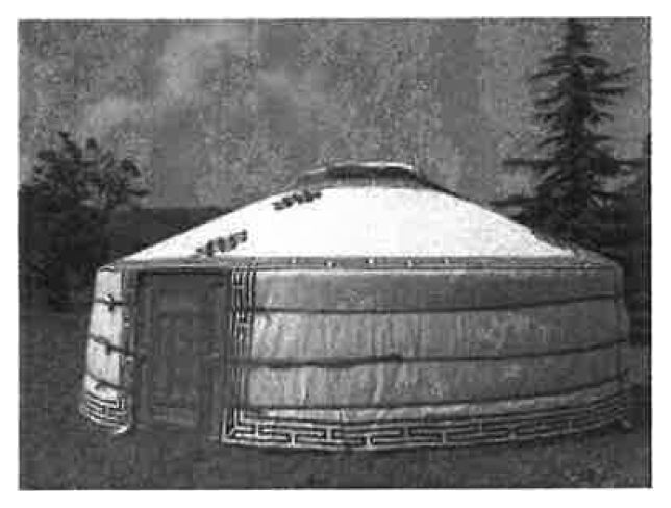
\includegraphics[width=4.5cm]{yourte}&
\psset{unit=0.9cm}
\begin{pspicture}(8.5,5)
%\psgrid
\scalebox{.99}[0.15]{\psarc[linewidth=4pt](5.1,8.5){2}{180}{0}}%
\scalebox{.99}[0.15]{\psarc[linewidth=4pt,linestyle=dashed](5.1,8.5){2}{0}{180}}%
\scalebox{.99}[0.15]{\psarc[linewidth=4pt](5.1,15.5){2}{180}{0}}%
\scalebox{.99}[0.15]{\psarc[linewidth=4pt,linestyle=dashed](5.1,15.5){2}{0}{180}}%
\rput(3.75,4.8){On modélise cette yourte par un cylindre et}
\rput(0.9,4.4){un cône.}
\psline[linewidth=2pt](3,2.3)(5,3.6)(7,2.3)
\psline[linewidth=2pt](3,1.3)(3,2.3)
\psline[linewidth=2pt](7,1.3)(7,2.3)
\psline{<->}(2.6,1.3)(2.6,3.6)\uput[l](2.6,2.45){4,5 m}
\psline{<->}(3,0.6)(7,0.6)\uput[d](5,0.6){7 m}
\psline{<->}(7.4,1.3)(7.4,2.3)\uput[r](7.4,1.8){2,5 m}
\end{pspicture}\\ \hline
\end{tabular}
\end{center}

\begin{center}
\begin{tabular}{|l|}\hline
On rappelle les formules suivantes :\\

Aire du disque $= \pi \times \text{rayon}^2$\\
Volume du cylindre $= \pi \times \text{rayon}^2 \times \text{hauteur}$\\
Volume du cône $= \dfrac{1}{3} \pi \times \text{rayon}^2 \times \text{hauteur}$\\ \hline
\end{tabular}
\end{center}

\medskip

\begin{enumerate}
\item Montrer que l'appartement de Samia offre une plus petite surface au sol que celle de la yourte.
\item Calculer le volume de la yourte en m$^3$.
\item Sarnia réalise une maquette de cette yourte à l'échelle $\frac{1}{25}$.

Quelle est la hauteur de la maquette?
\end{enumerate}

\bigskip

